%% Data section
%% All numbers verified against: code/build_iv_v2.py, code/01_build_spine.R,
%%   code/02_add_roads.R, code/03_add_census.R, code/04_add_econ_census.R,
%%   code/06_merge_all.R, code/run_full_analysis.R, data/analysis/dc_analysis_v2.csv
%% Figures referenced: figures/engineer_share_over_time.pdf, figures/sample_distribution_full.pdf

\section{Data}
\label{sec:data}

The analysis links three bodies of data at the district-year level: administrative
records on the careers of individual IAS officers, district-level measures of
programme delivery, and district demographic and economic characteristics. Officer
career histories are drawn from spells beginning as early as 1985, but the linked
estimation panel is constrained by the earliest outcome series (night-time
luminosity, described below) to begin in 1994; the usable district-year panel
therefore spans \textbf{1994--2008}, not the full 1985--2008 range over which officer
postings are observed. This section describes each source, the construction of the
estimation panel, and the coverage limitations that bear on interpretation.

\subsection{Officer Career Records}
\label{sec:data-officers}

Officer-level information is drawn from the SUPREMO administrative records
maintained by the Department of Personnel and Training, which document the service
histories of the universe of IAS officers: 13,570 officer profiles, of which 12,676
(93.4\%) carry at least one education record. For each officer I observe the entry
cohort, the assigned state cadre, the educational qualification recorded at entry,
and the complete sequence of postings held over the career, each with a start and
end date. The posting histories permit two constructions central to the empirical
strategy. First, they identify, for every district and year, the officer serving as
District Collector, yielding the district-year panel of Collector assignments.
Second, they identify, for every state and year, the set of officers available for
posting---those in the cadre not currently occupying a fixed-term assignment---which
constitutes the availability pool $\mathcal{A}_{st}$ underlying the queue-composition
instrument defined in Section~\ref{sec:identification}.

Educational qualifications are classified into three categories. The technical
category ($T$) comprises engineering, technology, and mathematics; the
social-science category ($S$) comprises economics, political science, law, and
public administration; and the residual category ($R$) comprises the natural
sciences, medicine, and the humanities. The technical--social-science contrast is
the object of the theoretical predictions in Section~\ref{sec:theory}; the residual
category is retained in all specifications without a directional prior.

Among the 12,676 officers with an education record, 11.4\% classify as technical,
32.2\% as social science, 21.6\% as residual, and the remaining 34.8\% carry no
classifiable subject code and are dropped. Roughly a quarter of officers (27.0\%)
list more than one qualification; where an officer's record contains qualifications
spanning more than one category, classification uses the qualification with the
highest \textit{Reference\_Value} in the source records---the officer's
most-advanced or most-recently-listed degree---breaking any remaining tie in favour
of the technical category, then social science, then residual. Restricting to the
officers who are eventually matched to a District Collector spell in the estimation
panel (Section~\ref{sec:data-coverage}), the composition shifts toward technical and
away from social science relative to the full officer population: 24.2\% technical,
46.6\% social science, and 29.2\% residual, consistent with the modest overrepresentation
of technical entrants in more recent allotment cohorts documented in
Table~\ref{tab:summary}.\footnote{Figure~\ref{fig:engineer_share} plots the technical
share of the active District Collector pool by year, showing this compositional
drift directly.}

\paragraph{Match rate.} Of the 8,483 District Collector-designation spells
identified in the officer experience records for 1985--2008 (held by 4,290 distinct
officers), 6,761 (79.7\%) are successfully linked to a Census (pc11) district
through the cadre--office name crosswalk; the remaining 20.3\% fail to match because
of spelling variants and historical revisions in office names, and because some
office entries predate the district boundaries fixed by the 2011 Census and cannot
be reconciled to a single pc11 district. Of the crosswalk-matched spells, 4,571
(67.6\%) are further linked to a district-year record in the outcome panel, for an
overall spell-level match rate of 53.9\% (4,571/8,483). The dominant reason for this
second-stage attrition is temporal, not administrative: the outcome panel is
anchored to the night-time-luminosity spine, whose earliest available year is 1994
(Section~\ref{sec:data-outcomes}), so any spell beginning before 1994---regardless of
crosswalk success---cannot be linked to an outcome. After dropping spells with
unclassifiable education and retaining the earliest spell observed in each
district-year, the estimation panel comprises 2,390 district-year observations.

Match success is close to balanced across educational categories for two of the
three outcomes: the night-time-luminosity and economic-census outcomes are
non-missing for 99.1--100\% of district-years in every education category. The
infrastructure outcome is less balanced---non-missing for 31.0\% of technical-officer
district-years versus 24.1\% (residual) and 22.5\% (social science)---but this gap
tracks a cohort-timing artefact rather than differential attrition on education:
technical officers enter the cadre on average roughly two years later than social
scientists (Table~\ref{tab:summary}), so a larger share of their District Collector
spells fall after 2001, when the road-completion series (below) becomes populated.
Because the road-completion regressions condition on district and year (or
state-by-year) fixed effects that absorb this timing pattern, the imbalance is not
expected to bias the education contrast, but it is a limitation worth flagging
directly rather than leaving implicit.

\subsection{Programme Outcomes}
\label{sec:data-outcomes}

The empirical strategy requires outcome measures that separate the two programme
classes of the theoretical framework---infrastructure and welfare---together with an
aggregate measure against which the composition prediction of
Proposition~\ref{prop:mix} can be tested.

\paragraph{Infrastructure.} Infrastructure delivery is measured by the rate of rural
road completion under the Pradhan Mantri Gram Sadak Yojana (PMGSY): the count of
roads completed in a district-year divided by completed road length (km),
constructed from the SHRUG shrid-level PMGSY release and aggregated to the
pc11 district by year using the shrid--district crosswalk. Completion dates in the
underlying data are recorded from 2000 onward, but coverage is thin before 2002 (six
district-years nationally in 2000, thirty-six in 2001, in the raw PMGSY district-year
panel prior to matching against District Collector spells); within the estimation
panel itself, where a match to a Collector spell is additionally required, only two
and seven district-years carry a non-missing value in 2000 and 2001 respectively. The
series becomes usably dense only from 2002, so regressions using this outcome are
restricted to 2001--2008 within the estimation panel, matching the roads-sample
windows referenced in Section~\ref{sec:results}. This outcome captures the
physical-capital dimension of
district administration in which technical training is predicted to confer
advantage.

\paragraph{Welfare.} Welfare delivery is measured by total employment per capita
from the quinquennial Economic Census (total workers across all establishments in a
district, divided by district population). The Economic Census is fielded
irregularly---rounds are available for 1990, 1998, 2005, and 2013---so each
panel-year is assigned the nearest completed round without look-ahead: 1990 values
for years before 1998, 1998 values for 1998--2004, 2005 values for 2005--2012, and
2013 values from 2013 onward. This is a step-function assignment, not an
interpolation, and it is the source of the outcome's near-complete coverage
(98.7--99.3\% non-missing by education category) despite the underlying survey being
sparse in time. Employment per capita, rather than a targeted transfer or
public-works outcome such as person-days under the rural employment guarantee
scheme, is used because the guarantee scheme was not enacted until 2006 and so falls
almost entirely outside the 1994--2008 estimation window; the Economic Census measure
is the broadest available proxy for the social-protection/livelihoods dimension of
district administration over the full sample period, in which social-science
training is predicted to confer advantage.

\paragraph{Aggregate activity.} Aggregate economic activity is measured by
inter-calibrated total night-time luminosity (DMSP-OLS, variable
\texttt{dmsp\_total\_light\_cal} from the SHRUG release) normalised by district
population, available annually for 1994--2013; VIIRS is not used, as its coverage
begins in 2012, after the estimation window closes. Twelve sample years (1994,
1997--2007) carry two simultaneous DMSP satellites, which are averaged within
district-year using the pre-calibrated series before use. Because luminosity
aggregates over both programme classes, Proposition~\ref{prop:mix} predicts that it
should display no systematic association with officer education type even when the
underlying programme-specific effects are non-zero; it therefore serves as a
falsification outcome rather than a primary one.

The three series differ materially in temporal coverage, which is why sample sizes
differ across the outcome-specific regressions in Section~\ref{sec:results}: night-time
luminosity is available for the entire 1994--2008 estimation window (2,390 of 2,390
district-year observations, 100\%); economic-census employment is available for
essentially the full window via the nearest-round assignment (2,365 of 2,390, 99.0\%);
and road completion is available for only 598 of 2,390 district-years (25.0\%),
concentrated in 2002--2008, because PMGSY record-keeping in the source data does not
extend meaningfully before 2000.

\subsection{District Characteristics}
\label{sec:data-districts}

District scale $N_j$ and baseline demographic controls---population, literacy, SC
and ST population shares---are drawn from the Census of India, 2001 and 2011 rounds.
Because the 2001 round is available at the shrid level and must be aggregated to
pc11 districts via the shrid--district crosswalk while the 2011 round is already
released at the pc11 district level, the two rounds are harmonised separately and
then combined into a single cross-sectional file. Each panel-year is assigned the
2001 values if the year precedes 2011 and the 2011 values otherwise; since the
estimation panel does not extend past 2008, every district-year in the analysis
sample in practice uses the 2001 Census baseline. These enter the analysis both as
the scale term in the production structure \eqref{eq:production} and as pre-period
baseline characteristics in the balance tests of Section~\ref{sec:validity}. The
counterfactual exercise in Section~\ref{sec:counterfactual} does not use a separate
sanctioned-target task-intensity measure; no such series is constructed in the
current data pipeline. Instead it takes district population $N_j$ as the scale term
and applies the instrumented comparative-advantage estimate directly, as described
in Section~\ref{sec:results-summary}.

\subsection{Estimation Panel and Coverage}
\label{sec:data-coverage}

The linked panel consists of 2,390 district-year observations across 518 districts
and 31 states, spanning 1994--2008. Each district contributes an average of 4.1
distinct Collectors (median 4) over the panel, with a mean recorded tenure of 16.6
months (median 15.0) and a median of 9 years of service at the time of posting---the
within-district rotation of officers of differing educational type across these
successive Collectors is the source of identifying variation. Figure~\ref{fig:sample_distribution}
shows the full distribution of District Collector spells by education group and
year; Figure~\ref{fig:engineer_share} shows the technical share of the active
Collector pool over time, which rises modestly across the sample period.

Two features of coverage bear on the interpretation of the estimates. First,
programme budgets are not observed at the district level: allocations under
centrally sponsored schemes are administratively confidential. The empirical
strategy accordingly does not condition on budgets directly. Instead, because
allocations are determined by centrally set formulas operating on observable
district characteristics, the district and state-by-year fixed effects absorb the
formula-driven component of budget variation, and identification of implementation
effectiveness proceeds from within-district variation in officer type conditional on
those effects. This is a limitation relative to a setting in which budgets were
observed, but it is one the institutional structure---in which the Collector
implements rather than allocates---renders tractable.

Second, the linkage of officer records to outcome series across the sample period is
incomplete, and the outcome series themselves differ in temporal coverage, as
detailed in Section~\ref{sec:data-outcomes}. The resulting estimates are therefore
directional rather than precisely estimated. This imprecision is anticipated by the
theoretical framework rather than incidental to it: Proposition~\ref{prop:atten}
establishes that estimates constructed from educational category---a noisy proxy for
the underlying capacity that the model places at the centre of the mechanism---are
attenuated toward zero by construction. The framework thus predicts small and
imprecisely estimated coefficients even where the underlying comparative-advantage
effect is substantial, and Section~\ref{sec:results} interprets the magnitude of the
estimates in that light.

%% ------------------------------------------------------------------
%% Figure placement notes (not floats -- to be inserted where the narrative
%% first references them, or gathered at the end of the section)
%%
%% \begin{figure}[htbp]
%%   \centering
%%   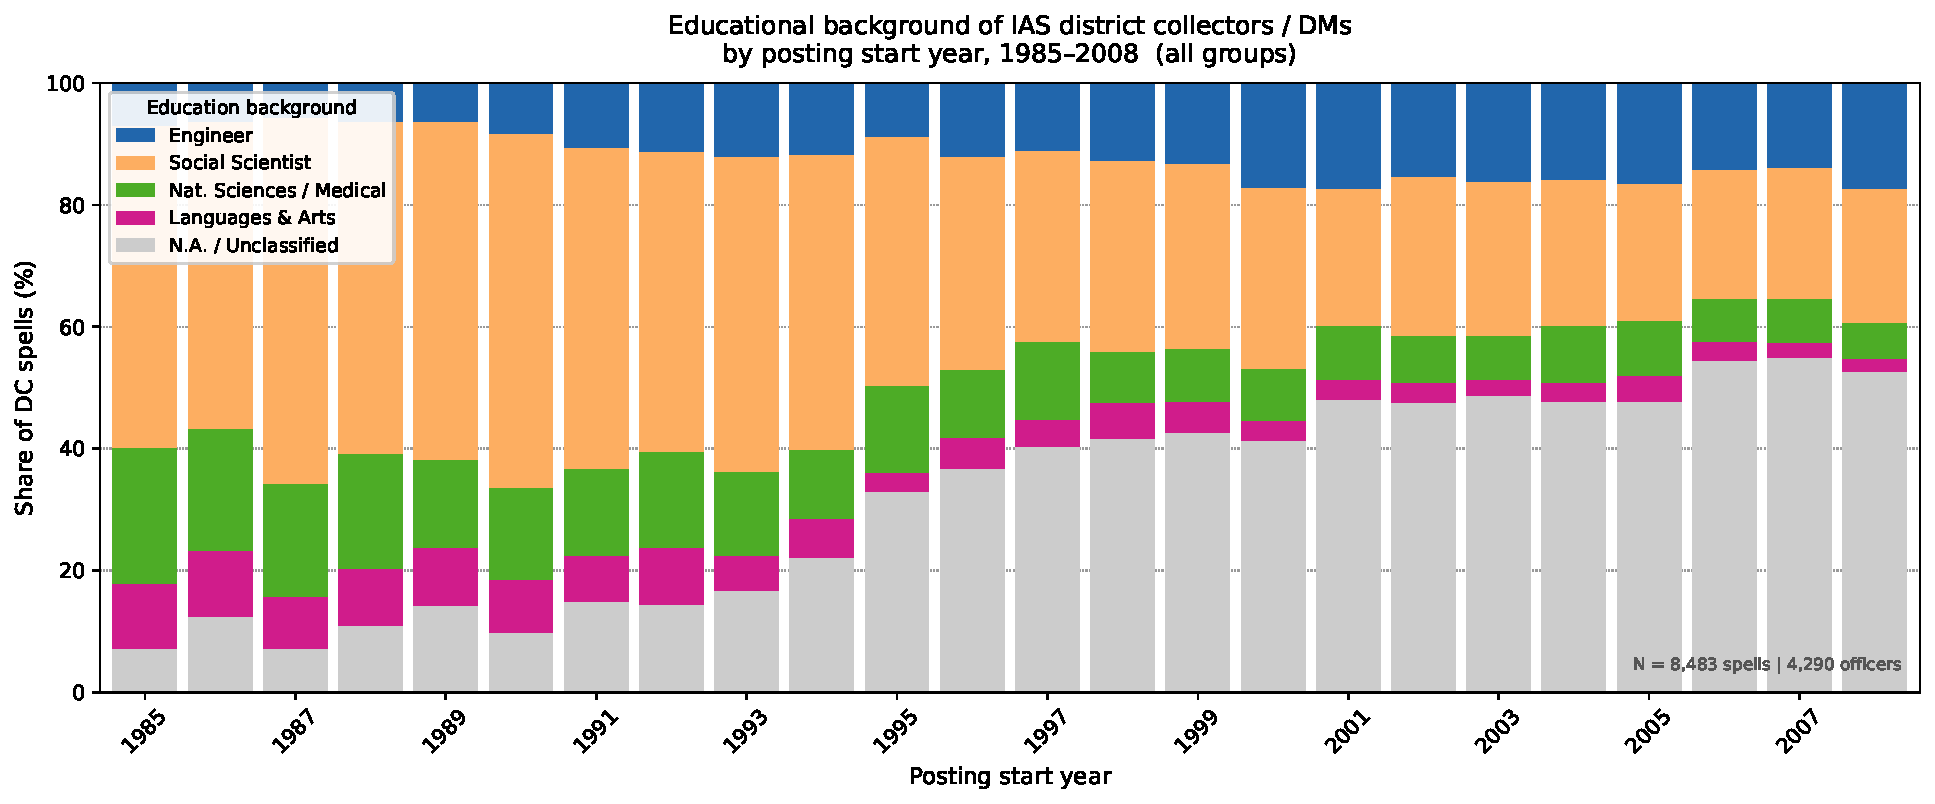
\includegraphics[width=0.8\textwidth]{figures/sample_distribution_full.pdf}
%%   \caption{Distribution of District Collector spells by education group, 1985--2008.}
%%   \label{fig:sample_distribution}
%% \end{figure}
%%
%% \begin{figure}[htbp]
%%   \centering
%%   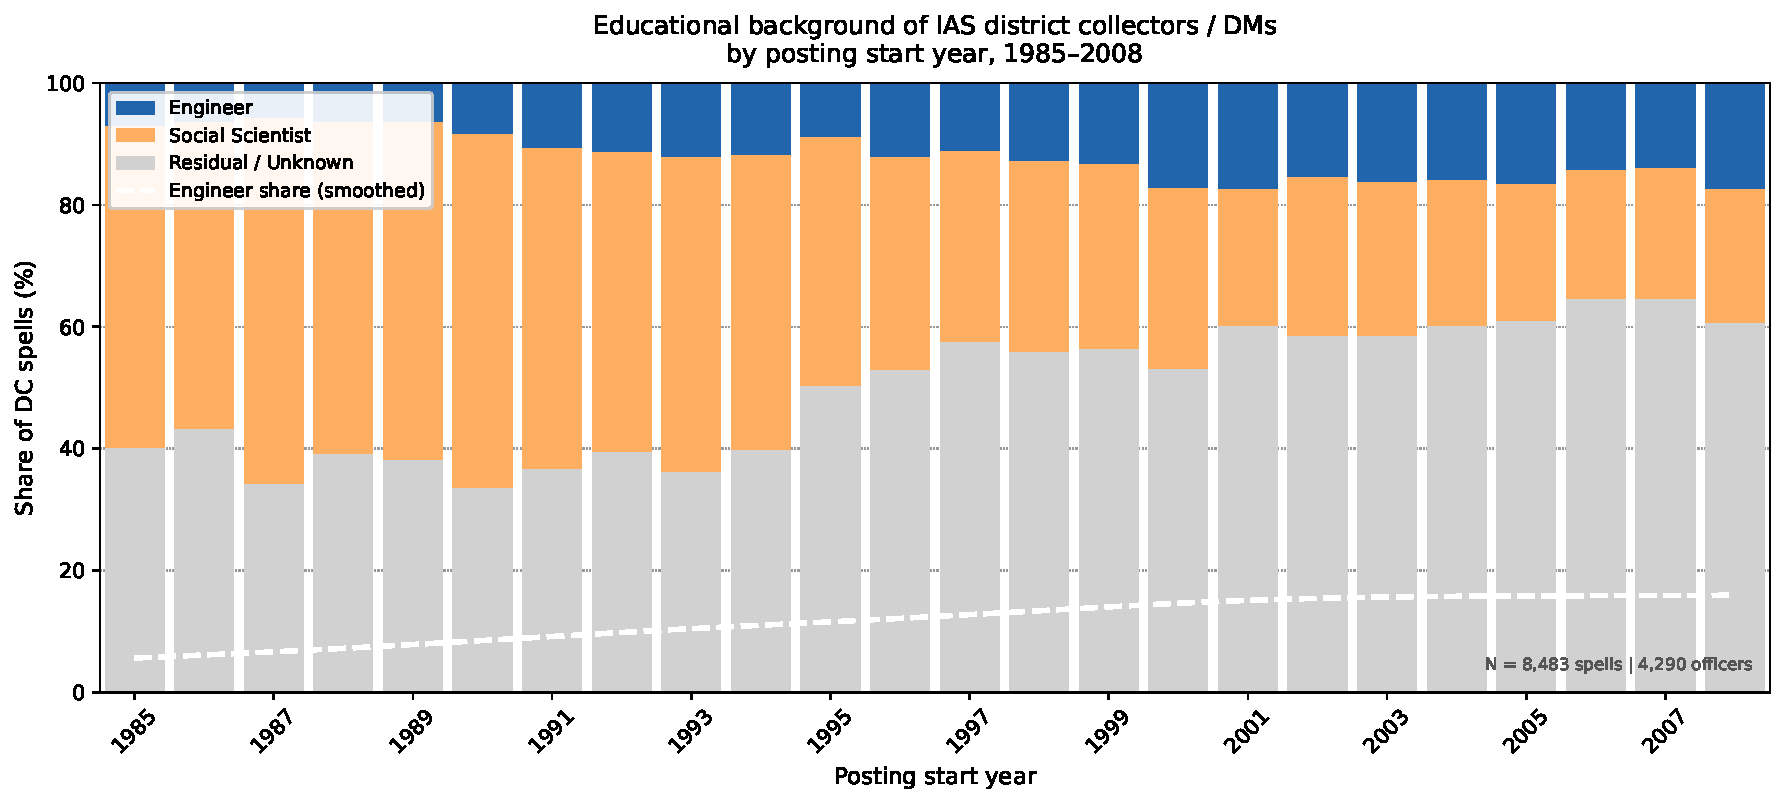
\includegraphics[width=0.8\textwidth]{figures/engineer_share_over_time.pdf}
%%   \caption{Technical (engineer) share of the active District Collector pool by year.}
%%   \label{fig:engineer_share}
%% \end{figure}
